\begin{pa} \label{PA:10.5} Suppose you are driving around in the
  $x$-$y$ plane in such a way that your position at time $t$ is given by the vector-valued
  function 
  $$
  \vr(t) = \langle x(t), y(t) \rangle = \langle 2-t^2, t^3 + 1\rangle.
  $$
  The path taken is shown on the left of Figure
  \ref{F:10.5.preview}.  

  \begin{figure}
    \begin{center}
      \includegraphics{figures/fig_10_5_preview_r.eps}
      \hspace*{20pt}
      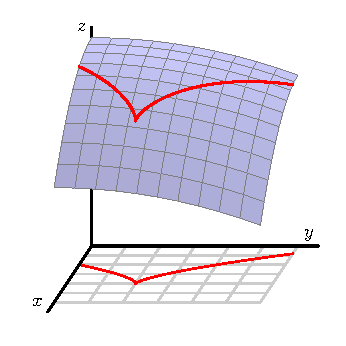
\includegraphics{figures/fig_10_5_preview_h.eps}
    \end{center}
    \caption{At left, your position in the plane; at right, the corresponding temperature.}
    \label{F:10.5.preview}
  \end{figure}
  Suppose, furthermore, that
  the temperature at a point in the plane is given by
  $$
  T(x,y) = 10 - \frac12x^2 -\frac15y^2,
  $$
  and note that the surface generated by $T$ is shown on the right of Figure \ref{F:10.5.preview}.  Therefore, as
  time passes, your position $(x(t), y(t))$ changes, and, as your position
  changes, the temperature $T(x,y)$ also changes.
  
  \ba
%\item What is your position at time $t=1$;  that is, what are the $x$-
 % and $y$-coordinates of your location?
%\item What is the temperature at this point?
\item The position function $\vr$ provides a parameterization $x = x(t)$ and $y = y(t)$ of the position at time $t$. By substituting $x(t)$ for $x$ and $y(t)$ for $y$ in the formula for $T$, we can write $T = T(x(t), y(t))$ as a function of $t$. Make these substitutions to write $T$ as a function of $t$ and then use the Chain Rule from single variable calculus to find $\frac{dT}{dt}$. (Do not do any algebra to simplify the derivative, either before taking the derivative, nor after.)
\item Now we want to understand how the result from part (a) can be obtained from $T$ as a multivariable function.  Recall from the previous section that small changes in $x$ and $y$ produce a change in $T$ that is approximated by 
\[\Delta T \approx  T_x\Delta x + T_y\Delta y.\]
The Chain Rule tells us about the instantaneous rate of change of $T$, and this can be found as  
\begin{equation} \label{eq:PA_10_5_1}
\lim_{\Delta t \to 0} \frac{\Delta T}{\Delta t} = \lim_{\Delta t \to 0} \frac{T_x \Delta x + T_y \Delta y}{\Delta t}.
\end{equation}
Use equation (\ref{eq:PA_10_5_1}) to explain why the instantaneous rate of change of $T$ that results from a change in $t$ is 
\begin{equation} \label{eq:PA_10_5_2}
\frac{dT}{dt} = \frac{\partial T}{\partial x} \frac{dx}{dt} + \frac{\partial T}{\partial y} \frac{dy}{dt}.
\end{equation} 
	\item  Using the original formulas for $T$, $x$, and $y$ in the problem statement, calculate all of the derivatives in Equation (\ref{eq:PA_10_5_2}) (with $T_x$ and $T_y$ in terms of $x$ and $y$, and $x'$ and $y'$ in terms of $t$), and hence write the right-hand side of Equation (\ref{eq:PA_10_5_2}) in terms of $x$, $y$, and $t$. 
	\item Compare the results of parts (a) and (c). Write a couple of sentences that identify specifically how each term in (c) relates to a corresponding terms in  (a). This connection between parts (a) and (c) provides a multivariable version of the Chain Rule. 
  \ea

\end{pa} 

\begin{activitySolution} 
  \ba
\item With $x(t) = 2-t^2$ and $y(t) = t^3+1$ we have 
\[T(x(t),y(t)) = 10-\frac{1}{2}\left(2-t^2\right)^2-\frac{1}{5}\left(t^3+1\right)^2.\]
So 
\[\frac{dT}{dt} = -\frac{1}{2}(2)\left(2-t^2\right)(-2t)-\frac{1}{5}(2)\left(t^3+1\right)(3t^2).\]

\item Since $\lim_{\Delta t \to 0} \frac{\Delta T}{\Delta t} = \frac{dT}{dt}$ and $T_x$ and $T_y$ don't depend on $\Delta t$, we have 
\begin{align*}
\lim_{\Delta t \to 0} \frac{T_x \Delta x + T_y \Delta y}{\Delta t} &= T_x \lim_{\Delta t \to 0} \frac{\Delta x}{\Delta t} + T_y  \lim_{\Delta t \to 0} \frac{\Delta y}{\Delta t} \\
	&= T_x \frac{dx}{dt} + T_y \frac{dy}{dt} \\
	&= \frac{\partial T}{\partial x} \frac{dx}{dt} + \frac{\partial T}{\partial y} \frac{dy}{dt}.
\end{align*}

	\item  Straightforward calculations show that 
\[T_x(x,y) = -x, \ T_y(x,y) = -\frac{2}{5}y, \ \frac{dx}{dt} = -2t, \ \text{ and } \ \frac{dy}{dt} = 3t^2.\]
Then
\begin{align*}
\frac{dT}{dt} &= \frac{\partial T}{\partial x} \frac{dx}{dt} + \frac{\partial T}{\partial y} \frac{dy}{dt} \\
	&= (-x)(-2t) - \frac{2}{5}y(3t^2).
\end{align*}
	
	\item With $x=2-t^2$ and $y = t^3+1$, the results of parts (a) and (c) are the same. The terms $-x$ and $-\frac{2}{5}y$ in (c) agree with what we get when we differentiate the outermost functions in (a). We can see where the terms $-2t$ and $3t^2$ in part (c) come from using the Chain Rule in (a) when we differentiate the innermost functions. 
  \ea
\end{activitySolution}

\afterpa 